\item

\begin{enumerate}
\item Es handelt sich um eine Hyperbel, die um eine Einheit entlang der Ordinate nach oben verschoben ist. Da das Argument $x$ in zweiter Potenz vorkommt, befinden sich bei Äste der Hyperbel überhalb der Abzisse.
\item $\int\limits_1^2 |f(x)-1| \diff{x} = \int\limits_1^2 \frac{2}{x^2} \diff{x} = -\frac{2}{x} \Big|_1^2 = 1$
\end{enumerate}

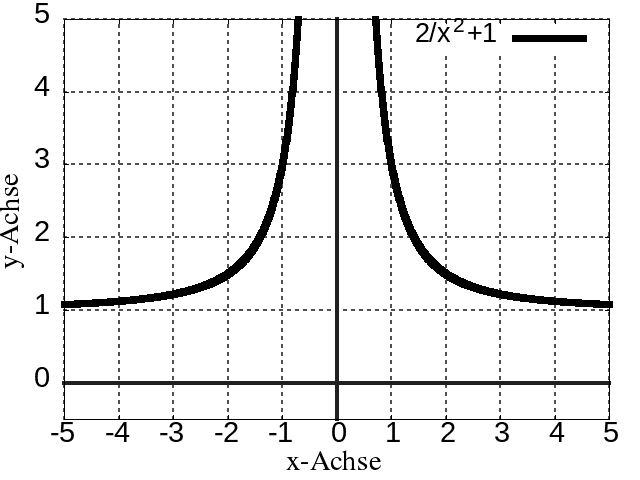
\includegraphics[width=0.5\textwidth]{../pool/ex-integral-6-img-a.png}
